
\section{Introduction to synthetic biology}

Synthetic biology aims at the rational design and construction of biological parts, devices, and systems in order to engineer organisms to perform new tasks~\autocite{Lu:2009ez, Andrianantoandro:2006bia}. A part is a basic unit, like a promoter or a ribosome binding site that when combined with other parts will make a functional unit, a device~\autocite{Heinemann:2006ht}. A device processes inputs, performs functions and produces outputs~\autocite{Andrianantoandro:2006bia}. A system comprises of a collection of devices.     

Emphasis is put on the use of engineering principles such as modularity, standardisation, use of predictive models and the separation of design and construction~\autocite{Agapakis:2009bt, Heinemann:2006ht}. A hierarchy similar to computer science is used, with cells, pathways and biochemical reactions acting as computers, modules and gates respectively~\autocite{Andrianantoandro:2006bia}. 
       
Numerous applications of synthetic biology have emerged, from altering existing metabolisms to producing synthetic drugs ~\autocite{Holtz:2010bm} or creating new synthetic life forms ~\autocite{Agapakis:2009bt}. Despite the successes there is still a lack of predictive power due to the stochasticity and lack of complete knowledge of the cellular environment ~\autocite{Andrianantoandro:2006bia}.

Synthetic biology is now entering an age where simple synthetic circuits have been built, such as toggle switches \autocite{Gardner:2000vha, Kramer:2004kq, Isaacs:2003ht, Ham:2008hh, Deans:2007cya, Friedland:2009ce}, oscillators~\autocite{Stricker:2008jqa, Fung:2005jd, Tigges:2009jx} and pulse generators~\autocite{Basu:2004gn}, but larger circuits have proven more difficult \autocite{XXX}. The leap from building low-level circuits to assembling them into complex networks has yet to be made successfully~\autocite{Lu:2009ez}, and predictable circuit behaviour remains challenging~\autocite{XXX}. Efforts to do so are plagued by intra-circuit crosstalk and incompatibility, as well as cellular noise, which can render synthetic networks non-functional \textit{in vivo} \autocite{XXX}. 

\section{System design in synthetic biology}

Creating synthetic devices that are robust to changing cellular contexts will be key to the success of synthetic biology. Unknown initial conditions and parameter values as well as the variability of the cellular environment, extracellular noise and crosstalk makes the majority of synthetic genetic devices non-functional~\autocite{Chen:2009ea}. Designing devices robust to this environment will lead to reliable behaviour of the systems.
When faced with a set of competing designs for a given genetic circuit, one is likely to choose the simplest possible model that can achieve the desired behaviour. However, simple systems are often the least robust. Feedback loops are well known key regulatory motifs~\autocite{Brandman:2005ci}. Negative feedback loops are essential for homeostasis and buffering~\autocite{Thomas:1995id} thus increasing robustness to extrinsic noise sources and positive feedback loops can generate multistationarity in a system~\autocite{Thomas:1995id}. Incorporating this kind of additional feedback interactions can make a design more robust and reliable. 
Maximising production is an important goal for a metabolic engineering project if it is to produce an economically viable substance~\autocite{Holtz:2010bm}. Network topologies and parameter values of different toggle switch designs are explored here in order to identify the design that maximises robustness and distance between steady states. This ensures the reliable production of the product with the greatest distance between the on and off states of the switch. 
 In the future, by selecting the system components accordingly, the parameter values can be adjusted \textit{in vivo}. For example, the parameter value corresponding to the translation initiation rate can be chosen by selecting the appropriate RBS sequence which given a nucleotide sequence will produce the desired rate~\autocite{Holtz:2010bm}, a method developed by~\textcite{Salis:2009gk}. Another method to tweak the parameter values \textit{in vivo} is to select the promoter to have the strength corresponding to the levels of gene expression and repression desired. Activity of each promoter can be measured and standardised~\autocite{Kelly:2009bj} making this process possible. For a system requiring more than one promoter, these can be efficiently selected from a promoter library using a genetic algorithm created by~\textcite{Wu:2011bq}. These standardised interchangeable components with known sequence and activity are what synthetic biology classes as BioBricks~\autocite{Kelly:2009bj,Canton:2008fv}. These can be selected and used to construct a desired system and replicate the parameter values found in the scan presented here.

The first computational approach for the tuning of robust synthetic networks was that of~\textcite{Batt:2007jl} where they examined the problem of finding a subset of the parameter set for which a given property was satisfied for all the parameters. \textcite{Chen:2009ea} used the fuzzy  dynamic game method to solve the minimax regulation design problem of synthetic genetic networks. In that method the worst case effect of all disturbances is minimised for a given network. An evolutionary algorithm has also been used to solve the robust design problem by evolving the parameters of the system in order to make it more robust to cellular disturbances by~\textcite{Chen:2011hj}. The added value of the methodology presented here is that the network structure in addition to the network parameters are adjusted to select a network that can robustly create the desired behaviour.	

\section{Introduction to Biochemical Modelling}
\subsection{Graphical representation of biochemical systems}

It is common to represent coupled biochemical reactions graphically. In a graph, as shown in Figure~\ref{fig:Toggle switch example}, nodes represent the species and the edges represent an interaction between the species it connects, in which a transcription factor directly affects the transcription of a gene~\autocite{alon:2007b}. An arrow at the end of an arc represents activation, i.e. that when the transcription factor binds to the promoter the rate of transcription of the gene increases. A flat line perpendicular to the arc at the end of an arc represents repression, i.e. that when the transcription factor binds to the promoter the rate of transcription of the gene decreases~\autocite{alon:2007b}.

\subsection{Deterministic and Stochastic modelling}

Modelling attempts to describe the elements and dynamics of the biochemical system of interest. It is a tool used for integrating knowledge and experimental data as well as for making predictions about the behaviour of the system~\autocite{wilkinson:2006}. When modelling a biochemical system it is generally assumed that the rates of a reaction are directly proportional to the concentration of the reactants, raised to the power of their stoichiometry~\autocite{wilkinson:2006}. This is known as mass-action kinetics and is used in this work to model the various systems.  
There are two main ways of modelling a system, deterministically and stochastically. Deterministic modelling utilises \acrfull{ode} and models the concentrations of the species (proteins or other molecules) by time-dependent variables~\autocite{deJong:2002ft}. Rate equations are used to model gene regulation where the rate of production of a species is a function of the concentrations of the other species~\autocite{deJong:2002ft}. When modelling deterministically the model is viewed as a system which, with sufficient knowledge of the system, its behaviour is entirely predictable. Nevertheless we are still a long way away from having complete knowledge of a system of interesting size~\autocite{wilkinson:2006}. Deterministic modelling also assumes a homogenous mixture where species concentrations vary continuously and deterministically, assumptions that often are not met \textit{in vivo}. A cell is spatially and temporally separated, due to small molecule numbers and fluctuations in the timing of processes~\autocite{deJong:2002ft}.  
   
In stochastic modelling, species are measured in discrete amounts rather than concentrations and a joint probability distribution is used to express the probability that at time \textit{t} the cell contains a number of molecules of each species~\autocite{deJong:2002ft}. It takes uncertainty into account and does not assume a homogenous mix. It is thus often more appropriate for modelling cellular systems, although more computationally intensive. In stochastic systems the Gillespie algorithm is widely used to simulate the time-evolution of the state of the system~\autocite{wilkinson:2006}. The algorithm, developed by~\textcite{Gillespie:1977ww} can be summarised in four steps:
\begin{enumerate}
\item Number of molecules in the system initialised
\item Two random numbers generated, one to determine which reaction will occur next and one to determine the time step
\item Time step increased and molecule counts updated according to Step 2 
\item Repeat from Step 2 until total simulation time reached
\end{enumerate}
   
 
\subsection{Steady state and stability}

In a steady state, the state of a system remains fixed. In non-linear systems, like the ones systems biology deals with, there is generally not an analytical solution thus the system has to be solved numerically. A stable steady state is defined as a fixed point whose nearby points approach the fixed point~\autocite{kaplan:1959}. This means that after a small perturbation the system will quickly return to the steady state. An unstable steady state is one which if the system is perturbed slightly then it moves away from the steady state~\autocite{konopka:2007}.    
 
 
\section{The genetic toggle switch}

One of the most common devices used in synthetic biology is the genetic toggle switch. A toggle switch consists of a set of transcription factors that mutually repress each other~\autocite{Gardner:2000vha}. Genetic switches play a major role in binary cell fate decisions like stem cell differentiation, as they are capable of exhibiting bistable behaviour. Bistability of a system is defined by the existence of two distinct phenotypic states but no intermediate state. Bistability is a property that is important in nature and a valuable resource to tap into in synthetic biology. It allows cells to alter their response to environmental cues and increases the overall population fitness by 'hedge-betting' the response of the population \autocite{XXX}. 

\subsection{Importance in natural systems}
In developmental processes, bistability ensures that the differentiating cell will follow one pathway, or the other, with no possible intermediate phenotypes. This is vital for the correct development of a cell in a specific pathway. One example is the trophectoderm differentiation pathway, in which a mutually inhibitory toggle switch exists between Oct3/4 and Cdx2. This determines whether an Embryonic Stem cell will differentiate into a Trophectoderm cell, if Cdx2 dominates the system, or an Inner Cell Mass cell if Oct3/4 dominates~\autocite{Niwa:2005fz}. Bistability is critical in this system as a cell must differentiate into either a trophectoderm cell or an inner cell mass cell, thus the signal to do so must be straightforward. In the case of the GATA1 and PU.1 toggle switch, the transcription factor pair controls the fate of the common myeloid progenitors, and the two possible differentiation paths are erythroid and myeloid blood cells~\autocite{Chickarmane:2009by}. The double-negative feedback loop created by the mutually repressive pair of transcription factors sustains the system in balance until an external stimulus causes one of the two transcription factors to increase in concentration. The increased concentration of one transcription factor causes the increased repression of the production of the antagonistic transcription factor, tipping the balance towards the dominance of the first transcription factor. The double negative feedback loop reinforces this dynamic and the system remains in the same state, until an external stimulus disturbs it~\autocite{FerrellJr:2002fh}.

\subsection{Uses in synthetic biology}
Despite their simplicity, toggle switches can be powerful building blocks with which to create complex responses in a synthetic network. They can be used in isolation or in tandem to create complex networks and signalling cascades. The toggle switch has been used for the regulation of mammalian gene expression~\autocite{Deans:2007cya, Kramer:2004kq}. Other synthetic applications of the toggle switch include the construction of a synthetic genetic clock~\autocite{Atkinson:2003tu}, of a predictable genetic timer~\autocite{Ellis:2009hka}, and the formation of biofilms in response to engineered stimuli~\autocite{Kobayashi:2004cv}. These applications are modifications of the classical toggle switch~\autocite{Gardner:2000vha}, and to our knowledge no application made of a cascade or collection of the switch has been successful. This would make more complex applications possible and could be used to solve real-life problems. For example, an analog-to-digital converter to translate external stimuli like the concentration of an inducer into an internal digital response, or programmable bacteria to move from point to point up different chemical gradients~\autocite{Lu:2009ez}. For a review on current circuits see~\autocite{Khalil:2010hm} and for possible future applications see~\autocite{Lu:2009ez}. This leap will be difficult to achieve before first being able to build robust and well characterised individual switches.

\subsection{Modelling the genetic toggle switch} 
The toggle switch motif has been studied extensively and there are numerous studies based on a number of different methods of modelling and analysis of the dynamics, including both deterministic and stochastic approaches. Deterministic modelling utilises ordinary differential equations (ODE) and models the concentrations of the species (proteins or other molecules) by time-dependent variables~\autocite{deJong:2002ft}. When modelling deterministically the model is viewed as a system whose behaviour is entirely predictable, given sufficient knowledge. In stochastic modelling, species are measured in discrete amounts rather than concentrations and a joint probability distribution is used to express the probability that at time \textit{t} the cell contains a number of molecules of each species~\autocite{deJong:2002ft,Wilkinson:2006}. It takes uncertainty into account and is thus often more appropriate for modelling cellular systems, although more computationally expensive. In stochastic systems the Gillespie algorithm is widely used to simulate the time-evolution of the state of the system~\autocite{Warren:2005kea}.
\par
The conclusions drawn about the stability and robustness of the toggle switch also vary between the different modelling approaches. Numerous studies have concluded that cooperativity is a necessary condition for bistability to arise~\autocite{Gardner:2000vha, Walczak:2005ds, Warren:2004baa, Warren:2005kea, Cherry:2000wi}. However, ~\textcite{Lipshtat:2006wb} found that stochastic effects can give rise to bistability even without cooperativity in three kinds of switch; the exclusive switch, in which there can only be one repressor bound at any one time, a switch in which there is degradation of bound repressors, and the switch in which free repressor proteins can form a complex, which renders them inactive as transcription factors~\autocite{Lipshtat:2006wb}. In another study, \textcite{Ma:2012dt} found that the stochastic fluctuations in a system involving such a small number of molecules, like the toggle switch, uncovers effects that can not be predicted by the fully deterministic case~\autocite{Ma:2012dt}. In their system, the toggle switch was found to be tristable, as small number effects render the third unstable steady state stable. \textcite{Biancalani:2015vya} identified multiplicative noise as the source of bistability in the stochastic case~\autocite{Biancalani:2015vya}. ~\textcite{Warren:2005kea} concluded that the exclusive switch is always more robust than the general switch, since the free energy barrier is higher~\autocite{Warren:2005kea}. A summary of the toggle switch models is shown in Table~\ref{tab:refs}. As is clear from above, there is yet to exist a consensus on the stability a switch is capable of, and the most appropriate method of modelling it. Different methods arrive at different conclusions, creating confusion on which behaviour to be expected by the experimentalist for even a simple system like the toggle switch, consisting of just two genes. The toggle switch cannot be used as a building block of larger, more complex systems until its behaviour can be predicted accurately. Until then, designing systems with predictable behaviour will be near impossible.


\begin{table}[]
\centering
\caption{Summary of stability for the toggle switch found via different modelling approaches}
\label{tab:refs}
\rotatebox{90}{
\begin{tabular}{@{}ccccccc@{}}
\toprule
                                        & \multicolumn{3}{c}{\textbf{Simple}}                                                                                                                                            & \multicolumn{3}{c}{\textbf{Double positive autoregulation}} \\ \midrule
                                        & \textit{Stability}                             & \textit{Reference} & \textit{Notes}                                                                                           & \textit{Stability}  & \textit{Reference}  & \textit{Notes}  \\  \midrule
\multirow{3}{*}{\textbf{Deterministic}} & Monostable                                     & \autocite{Loinger:2007vma}       & \begin{tabular}[c]{@{}c@{}}no cooperativity,\\ exclusive \& general\end{tabular}                         & Bistable            & \autocite{Guantes:2008gs}        &                 \\
                                        & \multirow{2}{*}{Bistable}                      & \autocite{Gardner:2000vha}       & copperativity \textgreater 2,                                                                            & Tristable           & \autocite{Guantes:2008gs}        &                 \\
                                        &                                                & \autocite{Loinger:2007vma}       & bound repressor degradation                                                                              & 4 steady steates    & \autocite{Guantes:2008gs}        &                 \\ \midrule
\multirow{7}{*}{\textbf{Stochastic}}    & Monostable                                     & \autocite{Loinger:2007vma}       & \begin{tabular}[c]{@{}c@{}}no cooperativity, \\ weak repression\end{tabular}                             & Tristable           & \autocite{Lu:2014kc}             &                 \\
                                        & \multirow{4}{*}{Bistable}                      & \autocite{Lu:2014kc}            &                                                                                                          &                     &                     &                 \\
                                        &                                                & \autocite{Biancalani:2015vya}    & \begin{tabular}[c]{@{}c@{}}exclusive,\\ controlled by noise strength\end{tabular}                        &                     &                     &                 \\
                                        &                                                & \autocite{Lipshtat:2006wb}      & no cooperativity                                                                                         &                     &                     &                 \\
                                        &                                                & \autocite{Loinger:2007vma}       & \begin{tabular}[c]{@{}c@{}}no cooperativity,\\ exclusive \& \\ bound repression degradation\end{tabular} &                     &                     &                 \\
                                        & \multicolumn{1}{l}{\multirow{2}{*}{Tristable}} & \autocite{Loinger:2007vma}       & \begin{tabular}[c]{@{}c@{}}no cooperativity,\\ strong repression\end{tabular}                            &                     &                     &                 \\
                                        & \multicolumn{1}{l}{}                           & \autocite{Ma:2012dt}           &                                                                                                          &                     &                     &                 \\ \bottomrule 
\end{tabular}
}
\end{table} 
\clearpage



\section{Introduction to Bayesian statistics}

\begin{align*}
p(\theta|x) &= \frac{p(x|\theta)p(\theta)} {\displaystyle \int p(x|\theta)p(\theta)d\theta\frac{p(x|\theta)p(\theta)}{p(x)}}
\end{align*}

because
\begin{align*}
p(x)p(\theta|x) &= p(\theta)p(x|\theta)
\end{align*}

where $p(x|\theta)$ is the likelihood, $p(\theta)$ is the prior, and $\displaystyle \int p(x|\theta)p(\theta)d\theta$ is the evidence. This is the normalisation. 

Bayes factor: 
\begin{align*}
B_{12} = \frac{\displaystyle \int p(x|\theta, M_1)p(\theta, M_1)d\theta}{\displaystyle \int p(x|\theta, M_2)p(\theta, M_2)d\theta}
\end{align*}


In our case, O is the objective, and D is the design. Therefore:

\begin{align*}
p(O|D_1) = \int p(O|\theta,D_1)p(\theta|D_1)d\theta,
\end{align*}



This is the robustness, or evidence or marginal likelihood

\begin{align*}
p(O|D_1) &= \displaystyle \int p(O|\theta,D_1)p(\theta|D_1)d\theta, \\
p(O|D_1) &= \displaystyle \iiint_{\underline{\Theta}} p(O|\underline{\Theta})p(\underline{\Theta}|D_1)d\underline{\Theta}
\end{align*}

where $\underline{\Theta} = \{ \theta_1, \theta_2,\theta_3 \}$ 

Assuming the prior is uniform, and $a=0$:

\begin{align*}
p(O|D_1) &= \displaystyle \iiint_{\underline{\Theta}} p(O|\underline{\Theta})\frac{1}{b_1}\frac{1}{b_2}\frac{1}{b_3}d\underline{\Theta} \\
p(O|D_1) &= \frac{1}{b_1}\frac{1}{b_2}\frac{1}{b_3} \displaystyle \iiint_{\underline{\Theta}}p(O|\underline{\Theta})d\underline{\Theta}
\end{align*}


Assuming uniform likelihood:
\begin{align*}
p(O|D_1) &= \frac{1}{b_1}\frac{1}{b_2}\frac{1}{b_3} \displaystyle \iiint_{\underline{\Theta}_F}1d\theta_1\theta_2\theta_3+\frac{1}{b_1}\frac{1}{b_2}\frac{1}{b_3} \displaystyle \iiint_{\underline{\Theta}_F}Od\underline{\Theta}
\end{align*}


\subsection{Bayes' theorem}
\subsection{Bayesian inference}
\subsection{Model checking}
\subsection{Prior selection}

%\section{Background}
A circuit must be robust to a fluctuating cellular environment and its response and sensitivity must be able to be fine tuned in order to orchestrate a network of circuits that function together. A robust circuit can tolerate the compound stochasticity that a chain of circuits brings, and fine tuning of its response and sensitivity enables the researcher to make it sensitive to an upstream signal as well as influence a downstream subsystem. Parts can be fine tuned by developing component libraries~\autocite{Lu:2009ez,}, but this will be of little use if the required parameter ranges for parts to make a functional complex network are unknown, and will only perpetuate the cycles of trial-and-error. A computational method to find the range of parameter values that will produce the behaviour of choice is crucial to the design process by enabling the informed selection of appropriate parts from the libraries. For example, if it is known that gene expression must be low for a given stability, one can select a weak promoter or a low copy plasmid for the desired construct. 

Both analytical and computational approaches have been deployed for the study of the toggle switch. Analytical approaches are limited to simpler models and thus require a number of assumptions to be made. The system under consideration has to be reduced to very few equations and parameters in order to make the system solvable. This requires assumptions to be made about the system that cannot always be justified, such as the~\acrfull{qssa}. The \acrshort{qssa} assumes that the binding/unbinding processes are much faster than any other process~\autocite{Loinger:2007vma}, thus the bound intermediate is assumed to always be in steady state. The \acrshort{qssa} assumption is met \textit{in vitro} but often does not hold \textit{in vivo} and its misuse can lead to large errors and incorrectly estimated parameters~\autocite{Pedersen:2007ke}. Moreover, it is generally not possible to solve even simple stochastic models analytically, and these methods are restricted to deterministic models. The computational and graph-theoretic approaches developed for the study of multistationarity generally focus on deciding on whether a given system is incapable of producing multiple steady states ~\autocite{Conradi:2007jo, Banaji:2010fh,Feliu:2013dz}. For example, ~\textcite{Feliu:2013dz} developed an approach using chemical reaction theory and generalised mass action modelling \autocite{Feliu:2013dz}. No approach exists that can handle both deterministic and stochastic systems in an integrated manner.

For this purpose, I developed a computational framework based on sequential Monte Carlo that takes a model and determines whether it is capable of producing a given number of (stable) steady states and the parameter space that gives rise to the behaviour. Uniquely, this can be done for both deterministic and stochastic models, and also complex models with many parameters, thus removing the need for simplifying assumptions. This framework can be used for comparing the conclusions drawn by various modelling approaches and thus provides a way to investigate appropriate abstractions. I have made this framework into a python package, called Stability Finder. 

I use this methodology to investigate genetic toggle switches and uncover the design principles behind making a bistable switch, as well as those necessary to make a tristable and a quadristable switch (4 steady states). I also demonstrate the ability of Stability Finder to examine more complex systems and examine the design principles of a three gene switch. The examples I used demonstrate that Stability Finder will be a valuable tool in the future design and construction of novel gene networks. 

%behind making a bistable switch, as well as those necessary to make a tristable switch. %We find that degradation rates of transcription factors are important for bistability, and that the addition of positive autoregulation can create tristable behaviour and also significantly more robust bistability when feedback strength is well balanced. Modelling transcription and translation allows us to conclude that transcriptional bursting can inhibit bistability, and also that bistability can occur even when the assumptions of time scale separation in the repressor dynamics are not met. We also examine the design principles behind the design of bistable versus tristable switches and highlight the importance of including stochastic dynamics when modelling these systems. Finally we demonstrate the ability of the framework to examine more complex systems and examine the design principles of a three gene switch. These examples demonstrate that StabilityFinder will be a valuable tool in the future design and construction of novel gene networks. 
\subsection{Model parametric Robustness}
\label{sec:rob_back}
During this thesis I define robustness as the ability of a system to retain its function despite parameter perturbations~\autocite{Stelling:2004wo}. The robustness of biological systems has been studied extensively~\autocite{Barkai:1997cd, Stelling:2004wo, Prill:2005fq, Kim:2006uk, Kitano:2007cp, Hafner:2009ct, Shinar:2010dd, ZamoraSillero:2011jw, Woods:2015vu}. and it is well known that feedback loops can increase the robustness of a system~\autocite{Becskei:2000ft,	 Doyle:2005ul}.

The robustness of a model can be calculated by dividing the volume of its functional region by the volume of its priors. This is a measure of the volume of the posterior distribution is compared to the priors. It comes from Bayes' rule that:

\begin{align}
	f(\theta|x) &= \frac{f(\theta)f(x|\theta)}{\int p(x|\theta)p(\theta)d\theta}
\end{align}

\noindent where $p(x|\theta)$ is the likelihood, $p(\theta)$ is the prior, and $\displaystyle \int p(x|\theta)p(\theta)d\theta$ is the evidence. The evidence is the normalisation  added so that the distribution integrates to 1. For a given model design D and objective O we define the functional region $F$ as the region within the prior where O is satisfied. So within the prior we can assign 1 to any region that falls within $F$ and 0 to any region outside that. 

\begin{align}
p(O|D_1) = \int p(O|\theta,D_1)p(\theta|D_1)d\theta,
\end{align}

\noindent For a design with three parameters this becomes:

\begin{align}
p(O|D_1) &= \displaystyle \iiint_{\underline{\Theta}} p(O|\underline{\Theta})p(\underline{\Theta}|D_1)d\underline{\Theta},
\end{align}

\noindent where $\underline{\Theta}$ is a vector containing the three parameters $ = \theta_1, \theta_2,\theta_3$. To calculate the robustness, or model evidence, we integrate this with respect to $\underline{\Theta}$. We assume  all parameters $\theta_1, \theta_2,\theta_3$ are uniform, $p(\underline{\Theta}|D_1) \sim U(a, b)$. If we assume a = 0 this integral becomes:

\begin{align}
p(O|D_1) &= \displaystyle \iiint_{\underline{\Theta}} p(O|\underline{\Theta})\frac{1}{b_1}\frac{1}{b_2}\frac{1}{b_3}d\underline{\Theta} \text{ , and }\\
p(O|D_1) &= \frac{1}{b_1}\frac{1}{b_2}\frac{1}{b_3} \displaystyle \iiint_{\underline{\Theta}}p(O|\underline{\Theta})d\underline{\Theta} \label{eq:1.6}
\end{align}

\noindent since $\frac{1}{b_1}\frac{1}{b_2}\frac{1}{b_3} $ is a constant. Then assuming that the likelihood is uniform Equation\ref{eq:1.6} becomes:

\begin{align}
p(O|D_1) &= \frac{1}{b_1}\frac{1}{b_2}\frac{1}{b_3} \bigg[\displaystyle \iiint_{\underline{\Theta}_F} 1 d\underline{\Theta} +\cancelto{0}{\displaystyle \iiint_{\underline{\Theta}_{\cancel{F} }} 0 d\underline{\Theta}}\bigg]  \\
\end{align}
\noindent since we assign 1 to any region within $F$ and 0 to any region outside it. This becomes:
\begin{align}
p(O|D_1) &= \overbrace{\frac{1}{b_1}\frac{1}{b_2}\frac{1}{b_3}}^{|P|} \underbrace{\displaystyle \iiint_{\underline{\Theta}_F} 1 d\underline{\Theta}}_{|F|}, \\
\therefore p(O|D_1) &= \frac{|F|}{|P|},
\end{align}
where |P| is the volume of the prior P and |F| the volume of the functional region F. Therefore, in the case where both the prior and the likelihood are uniform, the robustness $R$ of the design is the ratio of the volumes of the two.
%normal
%\begin{align*}
%p(O|\underline{\Theta}) = c \times exp\bigg(-\frac{(O-\mu)^2}{2\sigma^2}\bigg)
%\end{align*}

If on the other hand we assume the likelihood is multivariate normal, with priors remaining uniform, Equation\ref{eq:1.6} becomes: 
\begin{align}
p(O|D_1) &= \frac{1}{|P|}\iiint_{\underline{\Theta}}f(\underline{\Theta};\mu,\Sigma)d\underline{\Theta} \\%, & \parbox[c]{\Sigma = \det(\text{covariance matrix})} \\
\therefore p(O|D_1) &= \frac{1}{|P|}\underbrace{\times(2\pi)^\frac{k}{2}\times |\Sigma|^\frac{1}{2}}_{|F|} \\
\therefore p(O|D_1) &= \frac{|F|}{|P|},
\end{align}

We can use the Bayes' factor in order to compare the robustness between two model designs. The Bayes' factor is defined as follows:

\begin{align}
B_{ab} &= \frac{\displaystyle \int p(x|\theta, D_a)p(\theta, D_a)d\theta}{\displaystyle \int p(x|\theta, D_b)p(\theta, D_b)d\theta} \\
\therefore B_{ab} &= \frac{|Fa|}{|Pa|} / \frac{|Fb|}{|Pb|} \label{eq:final_bayes}
\end{align}

\noindent Therefore, we can use the ratio of the two robustness measures to calculate the Bayes' factor. If two models have a different number of parameters, the robustness of the system will only increase if |F| increases by more than the proportion by which |P| increased~\autocite{Woods:2015vu}. A model will be penalised for an additional if it does not increase the volume of the functional region by more than the volume that the added parameter added to the prior. This is true for nested models, where one model is wholly contained in the other. 



\section{\acrfull{abc}}
\subsection{\acrshort{abc} algorithms}

Stability Finder is based on a statistical inference method which combines \acrshort{abc} with \acrfull{smc}~\autocite{Toni:2009tr}. This simulation-based method uses an iterative process to arrive at a distribution of parameter values that can give rise to observed data or a desired system behaviour~\autocite{Barnes:2011hh}.

ABC methods are used for inferring the posterior distribution in cases where it is too computationally expensive to evaluate the likelihood function. Instead of calculating the likelihood, ABC methods simulate the data and then compare the simulated and observed data through a distance function~\autocite{Toni:2009tr}. Given the prior distribution $\pi(\theta)$ we can approximate the posterior distribution, $\pi(\theta\mid x)\propto f(x\mid\theta)\pi(\theta)$, where $f(x\mid\theta)$ is the likelihood of a parameter, $\theta$, given the data, $x$. There are a number of different variations of the ABC algorithm depending on how the the approximate posterior distribution is sampled. 

The simplest \acrshort{abc} algorithm is the \acrshort{abc} rejection sampler~\autocite{Pritchard:1999td}. In this method, parameters are sampled from the prior and data simulated through the data generating model. For each simulated data set, a distance from that of the desired behaviour is calculated, and if greater than a threshold, \textepsilon{}, the sample is rejected, otherwise it is accepted. 
\begin{algorithm}[H]

  \caption{ABC rejection algorithm}
 	\label{alg:ABC}
 \begin{algorithmic}[1]
    \Statex
	\State Sample a parameter vector \texttheta{} from prior $\pi(\theta)$
	\State Simulate the model given \texttheta{}
    \State Compare the simulated data with the desired data, using a distance function d and tolerance \textepsilon{}. if d $\leq$ \textepsilon{}, accept \texttheta{} 
   
  \end{algorithmic}
\end{algorithm}


\noindent The main disadvantage of this method is that if the prior distribution is very different from the posterior, the acceptance rate is very low~\autocite{Toni:2009tr}. An alternative method is the \acrshort{abc} \acrfull{mcmc} developed by~\textcite{Marjoram:2003up}. The disadvantage of this method is that if it gets stuck in an area of low probability it can be very slow to converge~\autocite{Sisson:wf}. 

The method used here is based on \acrlong{smc}, which avoids both issues faced by the rejection and \acrshort{mcmc} methods. It propagates the prior through a series of intermediate distributions in order to arrive at an approximation of the posterior. The tolerance, \textepsilon{}, for the distance of the simulated data to the desired data is made smaller at each iteration. When \textepsilon{} is sufficiently small, the result will approximate the posterior distribution~\autocite{Toni:2009tr}.  

%The desired behaviour of the system is used as the data to which the candidate model output is compared to \cite{Barnes:2011hh}. 
%Given a set of competing models, their associated prior estimates of their parameters and the design specifications, the algorithm is able to rank the models according to how well they describe the data and the posterior probabilities of the parameters \cite{Barnes:2011hh}. 

ABC SMC can identify the parameter values within a predefined range of values that can achieve the desired behaviour. It works by first sampling at random from the initial range set by the user, i.e. form the prior distribution of values. Each sample from the priors is called a particle. It then simulates the model given those values and compares that to the target behaviour. If the distance between the simulation and the target behaviour is greater than a predefined threshold distance \textepsilon{}, then the parameter values that produced that simulation are rejected. This is repeated for a predefined number of samples which are collectively referred to as a population. Each particle in a population has a weight associated with it, which represents the probability of it producing the desired behaviour. At subsequent iterations the new samples are obtained from the previous populations and the \textepsilon{} is set to smaller value, thus eventually reaching the desired behaviour. The algorithm proceeds as follows:

\begin{algorithm}[H]

  \caption{ABC SMC algorithm}
	\label{alg:ABC-SMC}
 \begin{algorithmic}[1]
    \Statex
    \State Select \textepsilon{} and set population t = 0
	\State Sample particles (\texttheta). If t = 0, sample from prior distributions (P). If t $\textgreater$ 0, sample particles from previous population.
	\State If t $\textgreater$ 0: Perturb each particle by $\pm$ half the range of the previous population (j) to obtain new perturbed population (i).
	\State Simulate each particle to obtain time course.
	\State Reject particles if d $\textgreater$ \textepsilon{}.
	\State Calculate the weight for each accepted particle. At the first population assign a weight equal to 1 for all particles. In subsequent populations the weight of a particle is equal to the probability of observing that particle divided by the sum of the probabilities of the particle arising from each of the particles in the previous population:

	\State $w_{t}^{(i)} = \begin{cases} 1, & \mbox{if } n = 0 \\\frac{P(\theta_{t}^{(i)})}{\sum_{j=1}^N w_{t-1}^{(j)} K_{t}(\theta_{t-1}^{(j)}, \theta_{t}^{(i)})}, & \mbox{if } n $\textgreater$  0. \end{cases}$

  \end{algorithmic}
\end{algorithm}


This algorithm is implemented on a simple example for illustration. A simple model was used, consisting of one species, $A$ converting to another, $B$. The model is described by two differential equations, where $A$ is the reactant and B the product, produced at a rate $p$. 

\begin{align}
\frac{d[B]}{dt} &= p[A] \\ 
\frac{d[A]}{dt} &= -p[A] 
\end{align}

The priors were set to $p \sim U(0, 10)$. Initial conditions for $A$ and $B$ were set to 1 and 0 respectively. The data to which the model was compared to was generated by simulating the same model with the parameter set to 1, as shown in Figure~\ref{fig:myABC true 1}.

\begin{figure*}[htbp]
    \begin{center}
    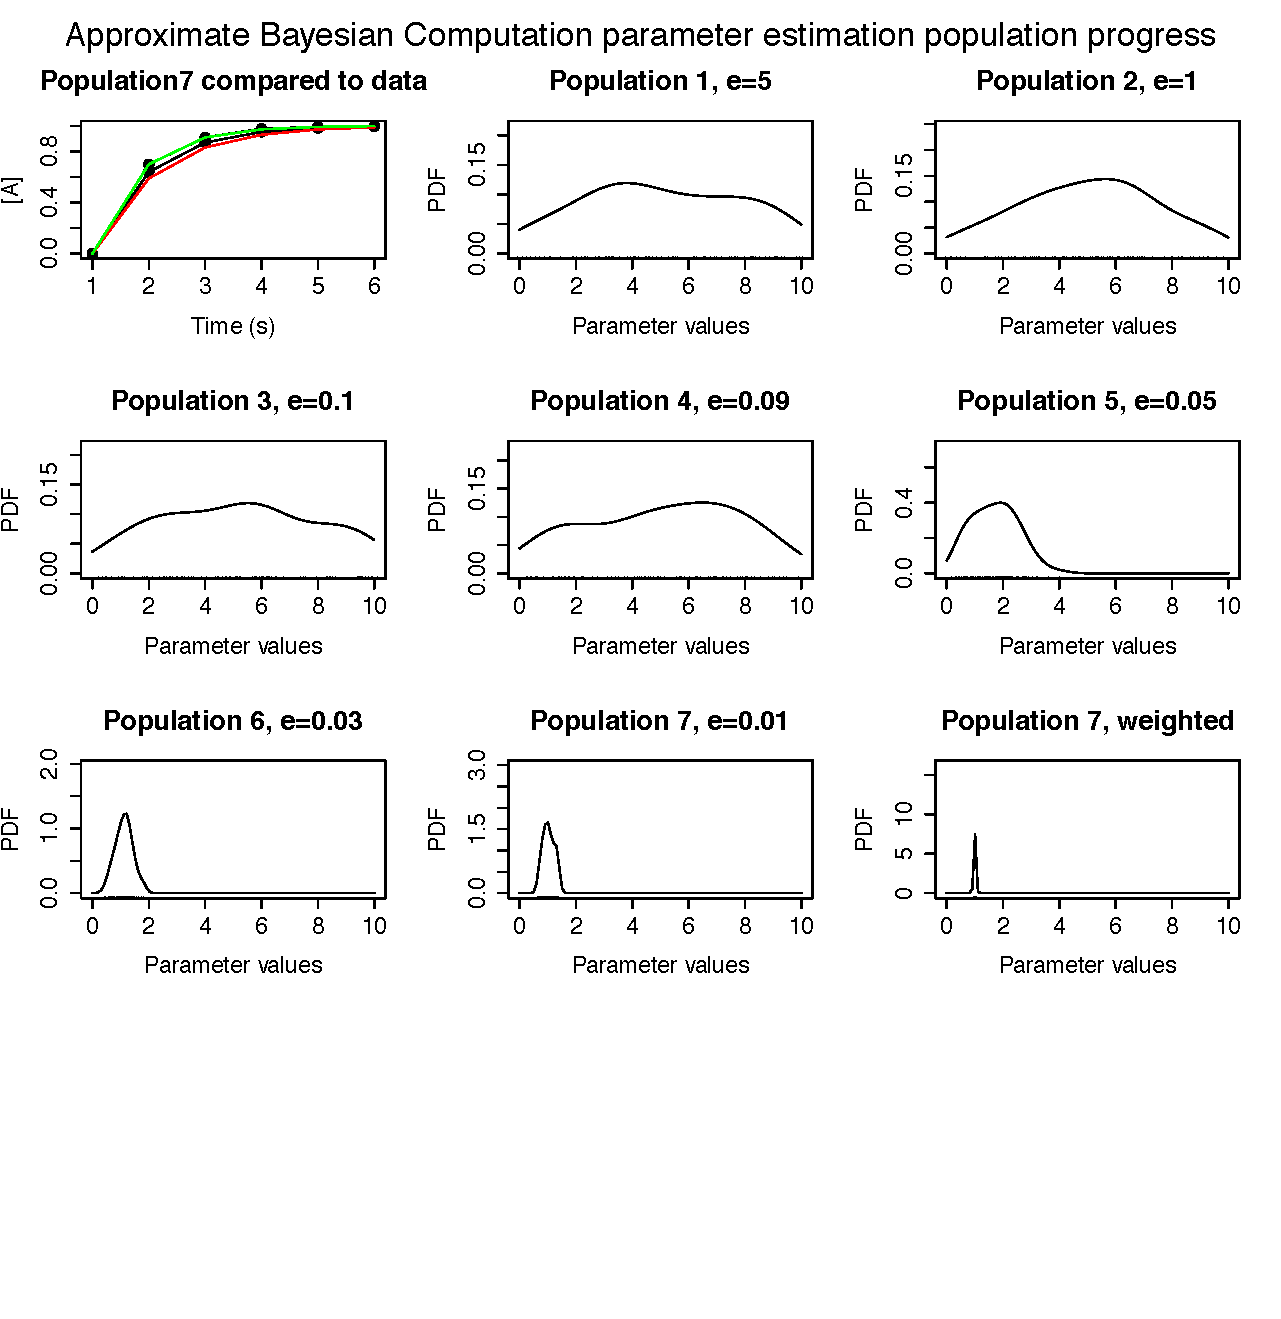
\includegraphics[scale=0.6]{chapterIntroduction/images/abcsmc_ex.pdf}
    \caption[\acrshort{abc} \acrshort{smc} example]{ABC SMC parameter inference. The posterior parameter is equal to 1 and its time course shown in red in the top left panel. The blue time course is that of the final population, green is the upper quartile and red is the lower quartile range of values. The progress of the selection process can be seen the \textepsilon schedule proceeds from the top left to the bottom right. The bottom far right panel is a density plot of \textepsilon = 0.01 with their weights taken into account.  }
    \label{fig:myABC true 1}
    \end{center}
\end{figure*}
\clearpage

Figure~\ref{fig:myABC true 1} demonstrates, using a simple example, that \acrshort{abc} \acrshort{smc} is capable of fitting a model to the data. During the course of 7 populations, the accepted distance \textepsilon{} of the simulated particles to the data is incrementally decreased. This leads to a final population where the distance of the data to the particles is very small, and there is a good agreement between the two. The algorithm concludes with a set of parameter values that produced this behaviour, which approximate the posterior distribution. The posterior distribution found in this model is in good agreement with the parameter value used to generate the data. This example successfully demonstrates the effectiveness of the \acrshort{abc} \acrshort{smc} algorithm in fitting models to data. 













